\documentclass[a4paper,12pt]{article}
\usepackage[russian]{babel}
\usepackage[T2A]{fontenc}
\usepackage[utf8]{inputenc}
\usepackage{geometry}
\usepackage{amsmath}
\usepackage{graphicx}
\usepackage{cancel}
\usepackage{float} 
\usepackage{xcolor}
\usepackage{array}
\usepackage{caption}
\usepackage{booktabs}
\usepackage{amssymb}
\usepackage{subcaption}
\usepackage{pgfplots}
\pgfplotsset{compat=1.18}
\usetikzlibrary{arrows.meta, matrix}
\usepackage{capt-of}
\usepackage{multirow}
\usepackage[siunitx]{circuitikz}
\usepackage[bottom]{footmisc}
\usepackage{tcolorbox}
\usepackage{nicematrix}
\usepackage{tikz}
\usetikzlibrary{positioning, arrows.meta}

% --- hyperref ОДИН РАЗ ---
\usepackage{hyperref}
\hypersetup{linktoc=page}
\hypersetup{
	colorlinks=true,
	linkcolor=red,
	citecolor=red,
	urlcolor=red,
	filecolor=red,
}

% --- Содержание ---
\usepackage{tocloft}
\usepackage{etoolbox}
\usepackage{hyperref}
\hypersetup{
	colorlinks=true,
	linkcolor=red,
	citecolor=red,
	urlcolor=red,
}

% Патчим \tableofcontents: текст строк — без ссылок и чёрный
% Это делается через замену \contentsline внутри TOC
\preto\tableofcontents{%
	\begingroup
	% Переопределяем contentsline так, чтобы текст был чёрным без ссылки,
	% а номер страницы — красной ссылкой
	\renewcommand{\contentsline}[4]{%
		\ifnum\pdfstrcmp{##1}{section}=0
		\vskip 4pt{\normalfont\color{black}##2}\nobreak\hfill
		{\normalfont\color{red}\hyperlink{##4}{##3}}\par
		\else\ifnum\pdfstrcmp{##1}{subsection}=0
		\vskip 2pt\hspace{1.5em}{\normalfont\color{black}##2}\nobreak\hfill
		{\normalfont\color{red}\hyperlink{##4}{##3}}\par
		\else
		\vskip 1pt\hspace{3em}{\normalfont\color{black}##2}\nobreak\hfill
		{\normalfont\color{red}\hyperlink{##4}{##3}}\par
		\fi\fi
	}%
}
\appto\tableofcontents{\endgroup}

% tocloft — только для отступов, без переопределения шрифтов
\usepackage{tocloft}

% --- Листинги ---
\usepackage{listings}

\definecolor{codebg}{RGB}{250,250,252}
\definecolor{linenumcolor}{RGB}{150,150,170}
\definecolor{mathblue}{RGB}{30,100,200}
\definecolor{mathorange}{RGB}{200,100,20}
\definecolor{matlabblue}{RGB}{0,0,200}
\definecolor{matlabgreen}{RGB}{30,130,30}
\definecolor{matlaborange}{RGB}{200,80,0}

\lstdefinelanguage{Mathematica}{
	keywords={Plot, Eigenvalues, MatrixExp, RiccatiSolve, IdentityMatrix,
		Inverse, Transpose, Simplify, Eigensystem, StateSpaceModel,
		ControllabilityMatrix, MatrixRank, Export, FileNameJoin,
		NotebookDirectory, ConstantArray, ZeroMatrix, NDSolve,
		Evaluate, LineLegend, Placed, Directive, Opacity, Filling,
		FillingStyle, PlotStyle, PlotLegends, PlotRange, Frame,
		Axes, FrameLabel, GridLines, GridLinesStyle, AspectRatio,
		Style, FontFamily, FontSize, Thick, Dashed, Dotted,
		DotDashed, RGBColor, GrayLevel, LegendLayout, LabelStyle,
		Subscript, Table, Do, Module, Block, If, True, False, Automatic},
	sensitive=true,
	morecomment=[s]{(*}{*)},
	morestring=[b]",
}

\lstdefinestyle{mma}{
	language=Mathematica,
	basicstyle=\ttfamily\small,
	keywordstyle=\color{mathblue}\bfseries,
	commentstyle=\color{linenumcolor}\itshape,
	stringstyle=\color{mathorange},
	numberstyle=\tiny\color{linenumcolor},
	numbers=left,
	numbersep=10pt,
	backgroundcolor=\color{codebg},
	frame=single,
	frameround=tttt,
	framesep=4pt,
	rulecolor=\color{mathblue!40},
	breaklines=true,
	tabsize=4,
	showstringspaces=false,
	captionpos=b,
	xleftmargin=15pt,
	xrightmargin=5pt,
}

\lstdefinestyle{matlab}{
	language=Matlab,
	basicstyle=\ttfamily\small,
	keywordstyle=\color{matlabblue}\bfseries,
	commentstyle=\color{matlabgreen}\itshape,
	stringstyle=\color{matlaborange},
	numberstyle=\tiny\color{linenumcolor},
	numbers=left,
	numbersep=10pt,
	backgroundcolor=\color{codebg},
	frame=single,
	frameround=tttt,
	framesep=4pt,
	rulecolor=\color{matlabblue!30},
	breaklines=true,
	tabsize=4,
	showstringspaces=false,
	captionpos=b,
	xleftmargin=15pt,
	xrightmargin=5pt,
	escapeinside={\%*}{*)},
	morekeywords={cvx_begin,cvx_end,sdp,variable,minimize,maximize},
}

\lstset{style=mma}

\renewcommand{\lstlistingname}{Листинг}
\DeclareCaptionFormat{redlisting}{#1\textcolor{red}{#2}#3}
\captionsetup[lstlisting]{format=redlisting}

\geometry{left=1.5cm, right=2cm, bottom=2cm, top=2cm}
\captionsetup[figure]{name=Рисунок}
\captionsetup[table]{name=Таблица}
\captionsetup{labelsep=endash}


\begin{document}
	
	\begin{titlepage}
		\centering
		
		\vspace*{0.5cm}
		{\small
			Министерство науки и высшего образования Российской Федерации\\[2pt]
			Федеральное государственное автономное образовательное учреждение\\
			высшего образования\\[2pt]
			\textbf{«Национальный исследовательский университет ИТМО»}\\
		}
		
		\vspace{0.8cm}
		\hrule height 0.8pt
		\vspace{0.3cm}
		
		{\large Факультет систем управления и робототехники}
		
		\vspace{0.3cm}
		\hrule height 0.4pt
		\vspace{2.5cm}
		
		{\Huge\bfseries ОТЧЁТ}\\[0.4cm]
		{\LARGE\bfseries о лабораторной работе}\\[0.8cm]
		
		\begin{tcolorbox}[
			colback=gray!4,
			colframe=gray!10,
			boxrule=0.8pt,
			arc=4pt,
			left=12pt, right=12pt, top=8pt, bottom=8pt
			]
			\centering
			{\large По дисциплине:\\[4pt]}
			{\large\bfseries «Теория опимального управления»}\\[10pt]
			{\large Тема:\\[4pt]}
			{\large\bfseries «Синтез оптимального регулятора для линейного стационарного объекта»} \\[10pt]
			{\large Поток: 1.3 \( \) Вариант: 18}
		\end{tcolorbox}
		
		\vspace{3cm}
		
		\begin{minipage}{0.45\textwidth}
			\raggedright
			{\large\bfseries Студент:}\\[4pt]
			Охрименко Е.\,Д.\\
		\end{minipage}
		\hfill
		\begin{minipage}{0.45\textwidth}
			\raggedleft
			{\large\bfseries Преподаватели:}\\[4pt]
			Герасимов Д.Н.\\
			Паромонов А. В.
		\end{minipage}
		
		\vfill
		\vspace{0.4cm}
		{\large Санкт-Петербург, 2026}
	\end{titlepage}
	
	\newpage
	\tableofcontents
	
	\newpage 
	\section{Постановка задачи}
	
	Требуется синтезировать оптимальный регулятор $u = -Kx$ для линейного стационарного объекта $\dot{x} = Ax + bu$, минимизирующий квадратичный функционал качества на бесконечном интервале времени:
	\[
	J = \int_{0}^{\infty} \left( x^T(\tau)Qx(\tau) + ru^2(\tau) \right) d\tau
	\]
	Расчет коэффициентов усиления $K$ необходимо произвести путем решения матричного уравнения Риккати с заменой:
	\[
	\begin{cases}
		A^TP + PA + Q - Pbr^{-1}b^TP = 0\\
		 K = r^{-1}b^TP
	\end{cases}
	\]
	Для моего варианта заданы следующие параметры системы:
	\[
	A = \begin{bmatrix} 0 & 1 \\ 5 & -3 \end{bmatrix} \qquad 
	b = \begin{bmatrix} 0 \\ 6 \end{bmatrix} \qquad 
	Q = \begin{bmatrix} 2 & 0 \\ 0 & 3 \end{bmatrix} \qquad 
	r = 2
	\]
	Моделирование замкнутой системы проводится при начальных условиях $x(0) = [1, 0]^T$. Дополнительно требуется исследовать робастность регулятора при отклонении матрицы $K$ и проанализировать влияние весовых параметров $Q$ и $r$ на качество переходного процесса.

	\newpage
	\section{Моделирование в Simulink}
	
	Структурная схема замкнутой системы реализована в среде \texttt{Simulink} и включает блоки объекта управления, оптимального регулятора $u=-Kx$ и вычисления критерия качества.
	
	\begin{figure}[H]
		\centering
		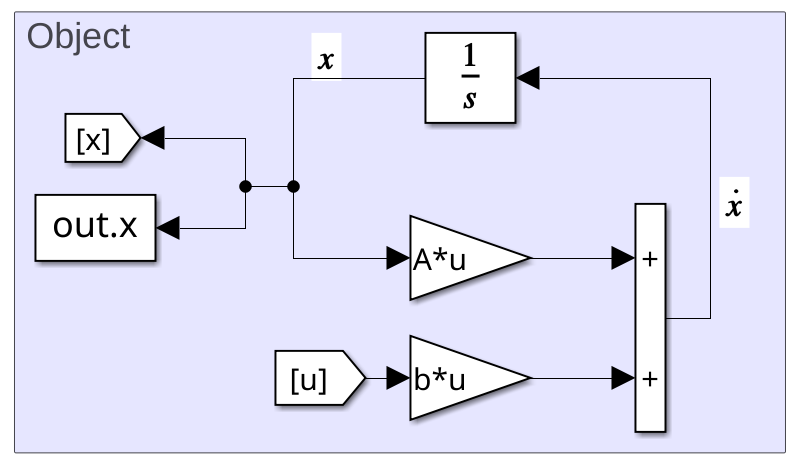
\includegraphics[width=0.5\textwidth]{../images/sim/obj.png}
		\caption{Схема моделирования объекта управления}
		\label{fig:sim_obj}
	\end{figure}
	
	\begin{figure}[H]
		\centering
		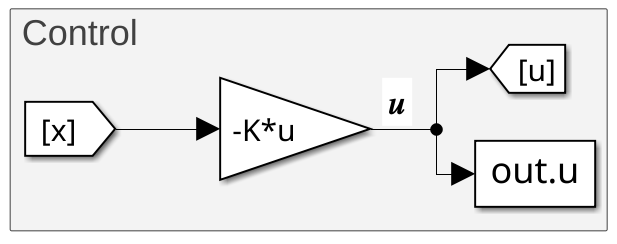
\includegraphics[width=0.45\textwidth]{../images/sim/Control.png}
		\caption{Блок формирования оптимального управления}
		\label{fig:sim_control}
	\end{figure}
	
	\begin{figure}[H]
		\centering
		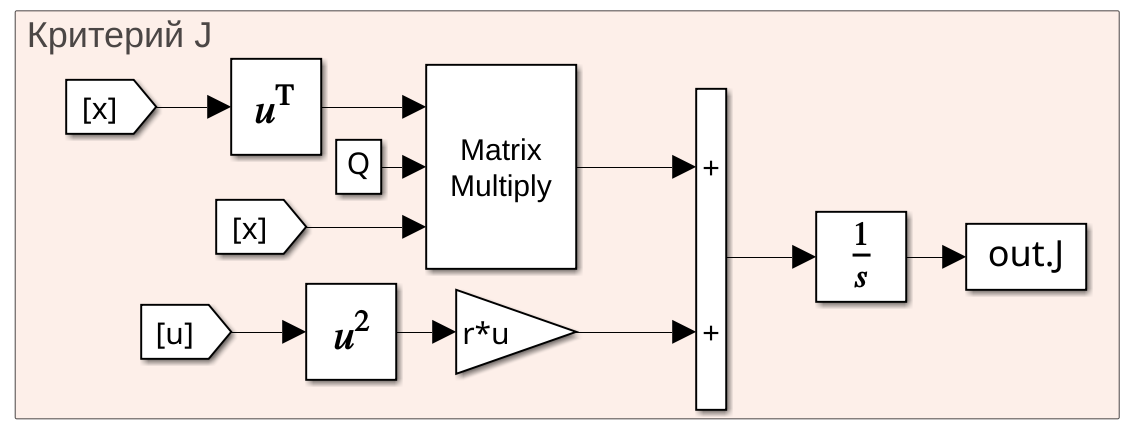
\includegraphics[width=0.7\textwidth]{../images/sim/J.png}
		\caption{Схема вычисления накопленного критерия качества $J(t)$}
		\label{fig:sim_J_block}
	\end{figure}




	
	
	
	
	
	\newpage
	\section{Синтез оптимального регулятора}
	 
	Синтезируем управление \(u = -K x\) при помощи матричного уравнения Риккати (листинг~\ref{lst:icare}). Полученная матрица регулятора:
	
	\[
	K = \begin{bmatrix}
		1.25 & 0.28
	\end{bmatrix}
	\]
	
	Собственные числа замкнутой системы:
	
	\[\sigma(A- b k) = \left\{-2.32 , -7.43\right\}\]
	
Аналитическое значение критерия качества для начальных условий \(x(0) = [1, 0]^T\) рассчитывается как квадратичная форма от матрицы \(P\):
\[
J_{\min} = x_0^T P x_0 = 
\begin{bmatrix} 1 & 0 \end{bmatrix}
\begin{bmatrix} 
	0.9698 & 0.1104 \\ 
	0.1104 & 0.2959 
\end{bmatrix}
\begin{bmatrix} 1 \\ 0 \end{bmatrix} 
= 0.9698
\]

	
	
	
	\begin{figure}[H]
		\centering
		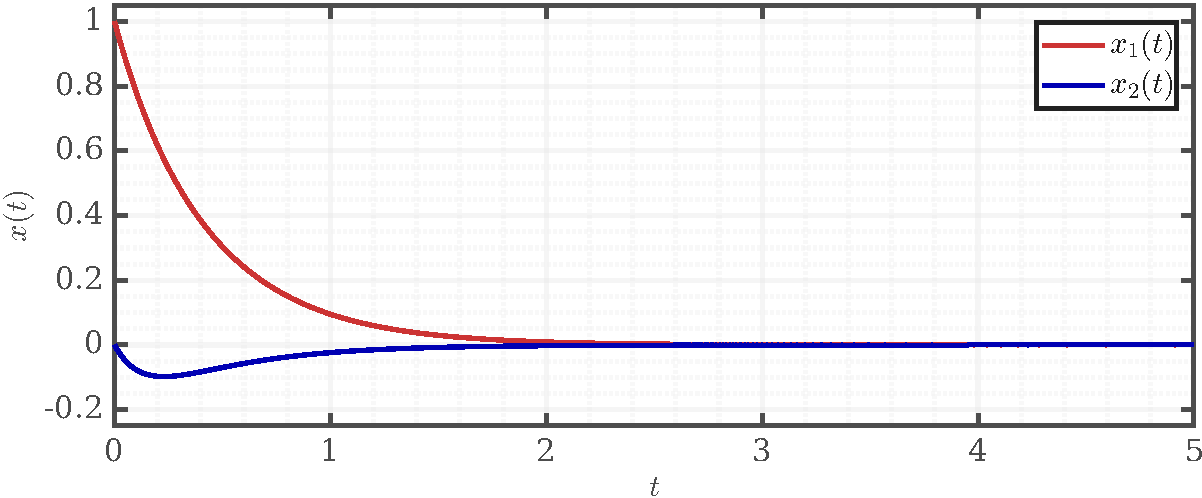
\includegraphics[width=0.65\textwidth]{../images/task2/x.pdf}
		\caption{Траектории состояния $x(t)$ при $x(0)=[1, 0]^T$}
		\label{fig:task3_x}
	\end{figure}
	
	\begin{figure}[H]
		\centering
		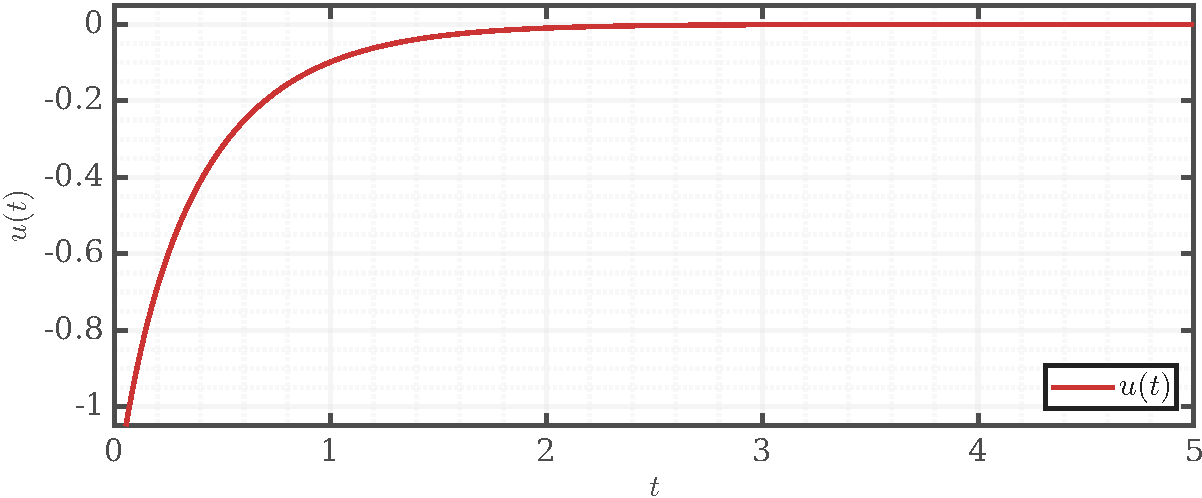
\includegraphics[width=0.65\textwidth]{../images/task2/u.pdf}
		\caption{Оптимальное управление $u(t)$}
		\label{fig:task3_u}
	\end{figure}
	
	\begin{figure}[H]
		\centering
		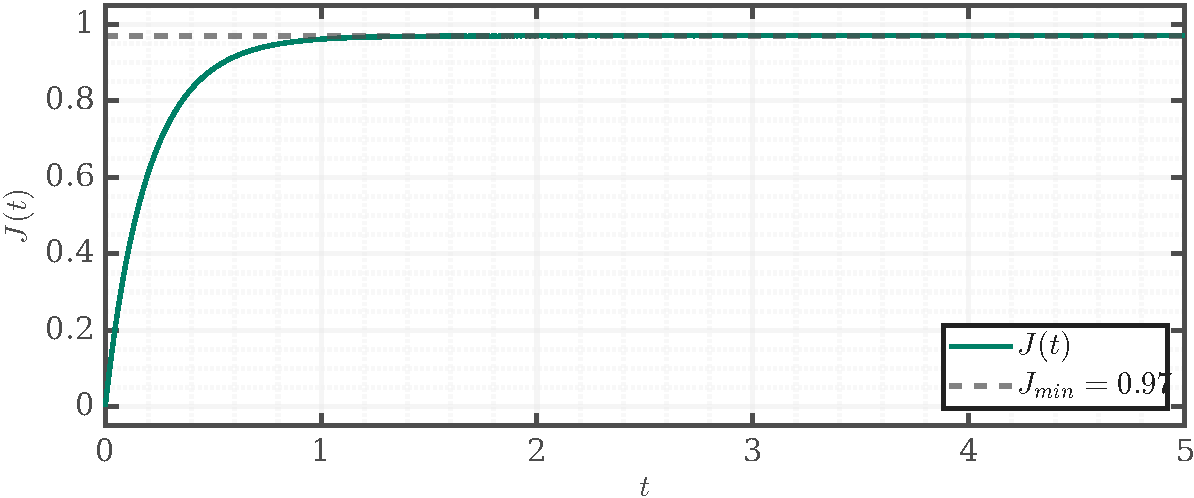
\includegraphics[width=0.65\textwidth]{../images/task2/J.pdf}
		\caption{Накопленный критерий качества $J(t)$ и его предельное значение $J_{min}$}
		\label{fig:task3_J}
	\end{figure}
	
	
	
	\newpage
	\section{Анализ робастности регулятора}
	
	Для оценки чувствительности синтезированного управления матрица коэффициентов усиления была отклонена на $15\%$ от оптимальных значений:
	\[
	K = \begin{bmatrix}
		1.06 & 0.72
	\end{bmatrix}
	\]
	
	Собственные числа замкнутой системы с отклоненным регулятором:
	\[
	\sigma(A - b K) = \{-2.0888, -6.6420\}
	\]

	
	\begin{figure}[H]
		\centering
		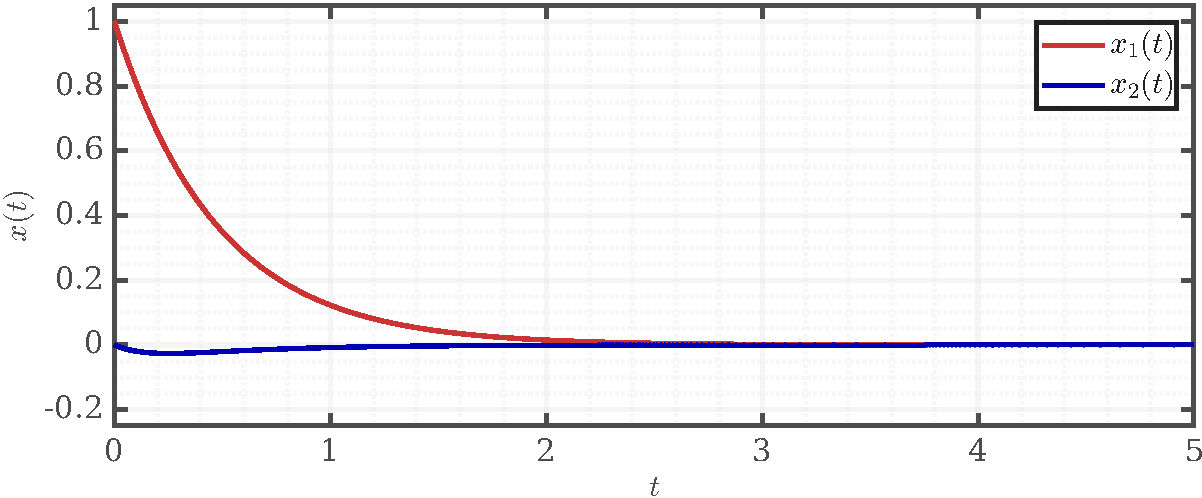
\includegraphics[width=0.65\textwidth]{../images/task3/x.pdf}
		\caption{Траектории состояния \(x(t)\) при отклонении \(K\) на \(10\%\)}
	\end{figure}
	
	\begin{figure}[H]
		\centering
		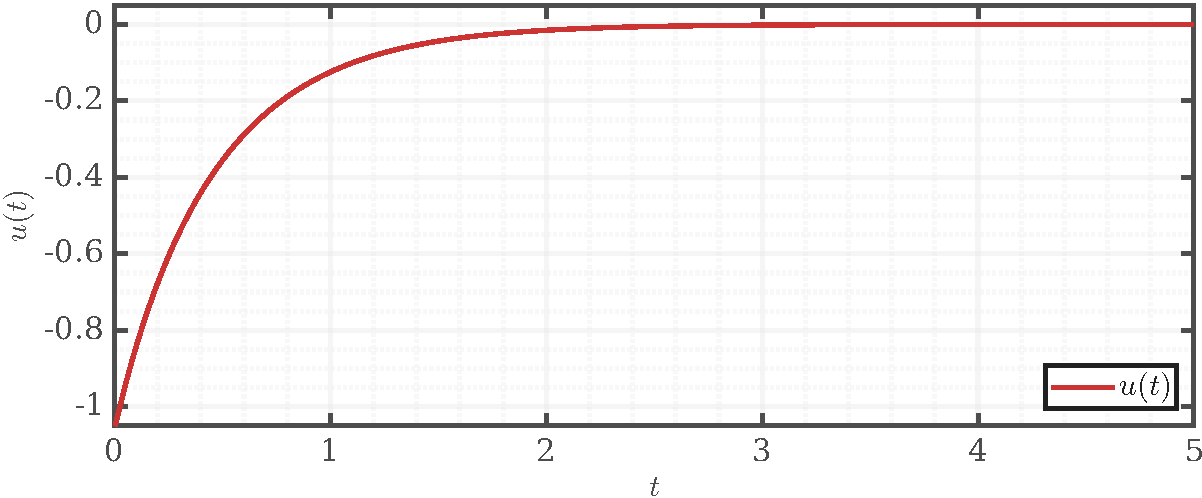
\includegraphics[width=0.65\textwidth]{../images/task3/u.pdf}
		\caption{Управляющее воздействие \(u(t)\) при отклонении \(K\)}
	\end{figure}
	
	\begin{figure}[H]
		\centering
		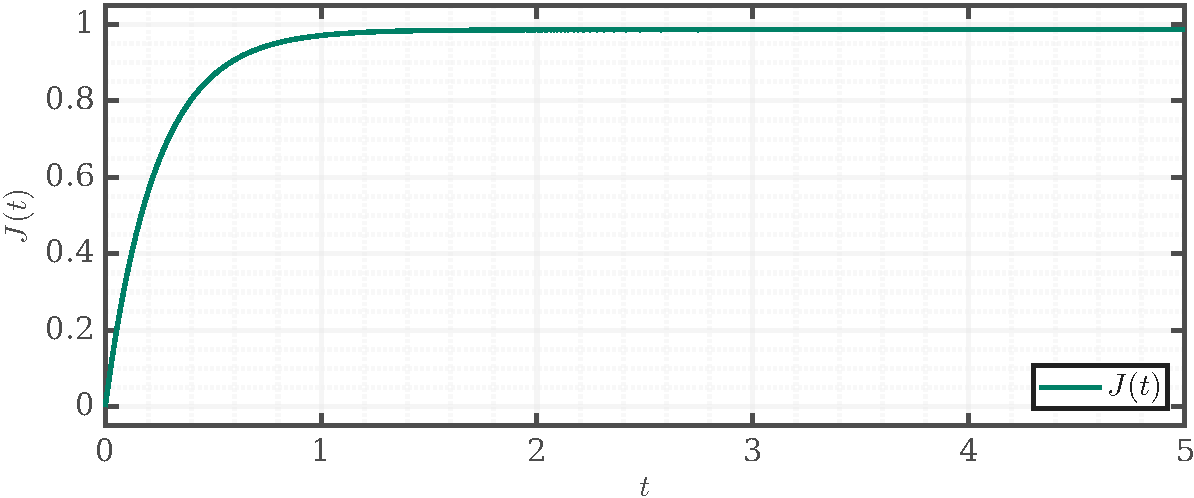
\includegraphics[width=0.65\textwidth]{../images/task3/J.pdf}
		\caption{Критерий качества \(J(t)\) при отклонении \(K\) и его предельное значение}
	\end{figure}
	
	
		
	Отрицательные действительные части собственных чисел подтверждают сохранение устойчивости системы. Переходные процессы также, как и в предыдущем эксперименте длятся примерно 2 секунды. Однако значение критерия качества возрастает по сравнению с оптимальным случаем.
	
	
	
	 
	
	\newpage
	\section{Анализ влияния весовых параметров}
	
	Проведено моделирование для трех наборов параметров $(Q, r)$. Результаты синтеза и значения критерия качества представлены в таблице~\ref{tab:lqr_params}.
	
	\begin{table}[H]
		\centering
		\caption{Параметры регулятора и критерий качества для различных весовых матриц}
		\label{tab:lqr_params}
		\renewcommand{\arraystretch}{1.2}
		\begin{tabular}{@{}lccc@{}}
			\toprule
			\textbf{Эксперимент} & \textbf{$K$} & \textbf{$\sigma(A-bK)$} & \textbf{$J_{\min}$} \\
			\midrule
			$2Q^*, \; r=4$      & $[1.2458, \; 0.8501]^T$ & $\{-2.317, \; -7.425\}$ & $1.9396$ \\
			$Q^*, \; r=10$      & $[0.9240, \; 0.3735]^T$ & $\{-1.817, \; -4.899\}$ & $2.9856$ \\
			$5Q^*, \; r=0.5$    & $[3.0933, \; 4.4764]^T$ & $\{-2.542, \; -29.026\}$& $2.0773$ \\
			\bottomrule
		\end{tabular}
	\end{table}
	
	Графики переходных процессов для каждого эксперимента приведены на рисунках~\ref{fig:exp_x}--\ref{fig:exp_J}.
	
	\begin{figure}[H]
		\centering
		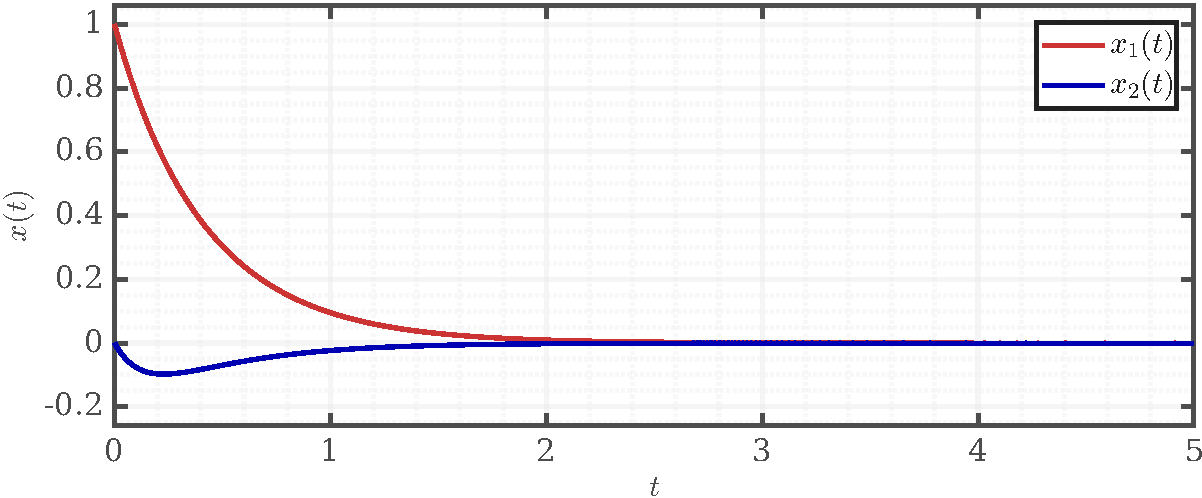
\includegraphics[width=0.65\textwidth]{../images/task4/x_1.pdf}
		\caption{Траектории состояния \(x(t)\): эксперимент 1 ($2Q^*, r=4$)}
		\label{fig:exp_x}
	\end{figure}
	
	\begin{figure}[H]
		\centering
		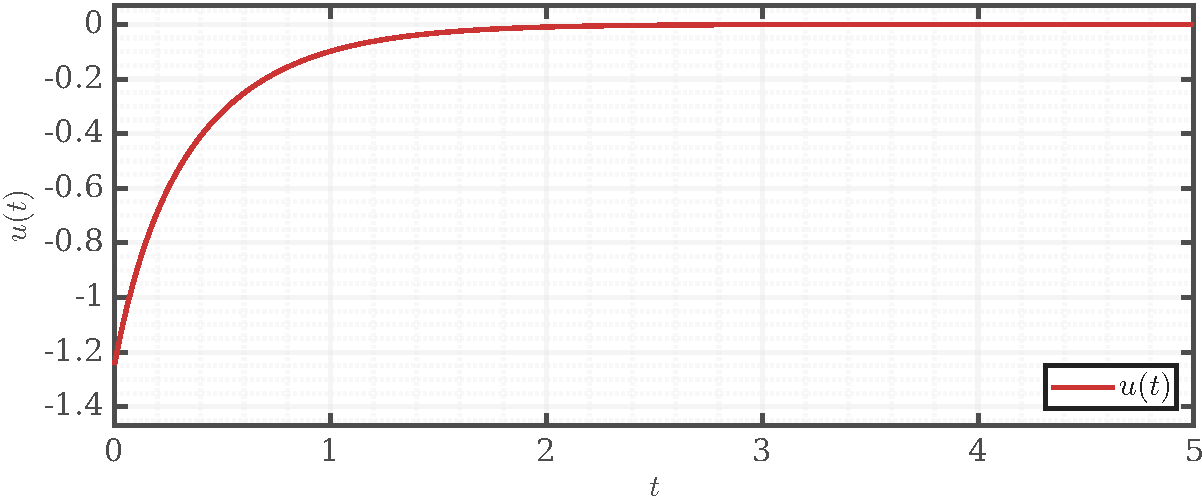
\includegraphics[width=0.65\textwidth]{../images/task4/u_1.pdf}
		\caption{Управление \(u(t)\): эксперимент 1 ($2Q^*, r=4$)}
		\label{fig:exp_u}
	\end{figure}
	
	\begin{figure}[H]
		\centering
		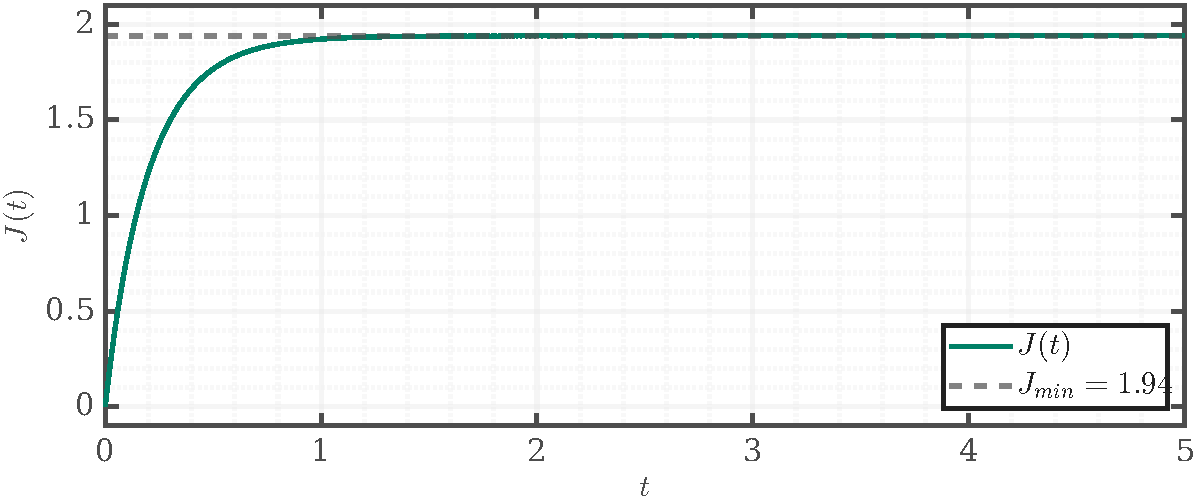
\includegraphics[width=0.65\textwidth]{../images/task4/J_1.pdf}
		\caption{Критерий качества \(J(t)\): эксперимент 1 ($2Q^*, r=4$)}
		\label{fig:exp_J}
	\end{figure}
	
	% --- Эксперимент 2 ---
	\begin{figure}[H]
		\centering
		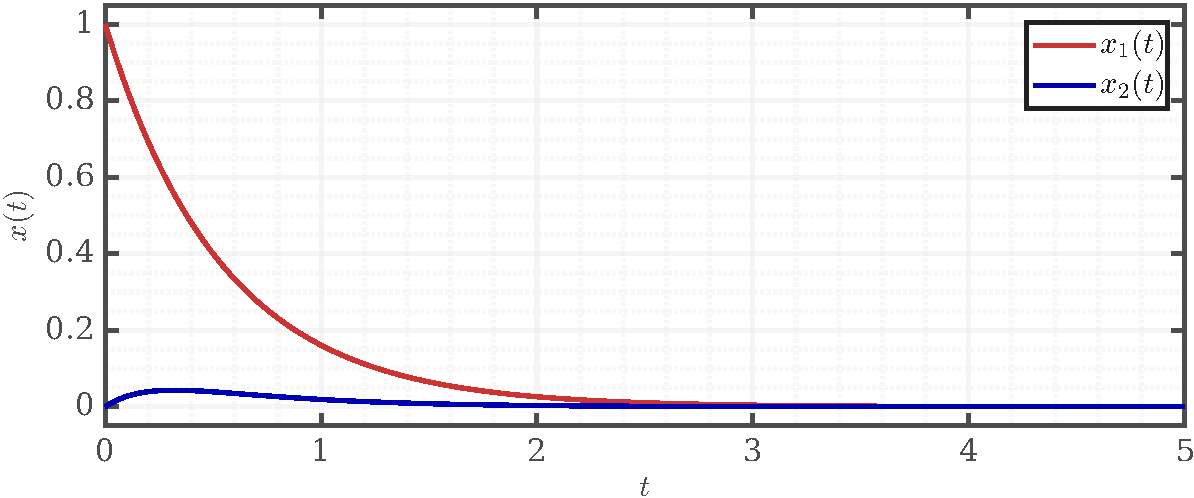
\includegraphics[width=0.65\textwidth]{../images/task4/x_2.pdf}
		\caption{Траектории состояния \(x(t)\): эксперимент 2 ($Q^*, r=10$)}
	\end{figure}
	
	\begin{figure}[H]
		\centering
		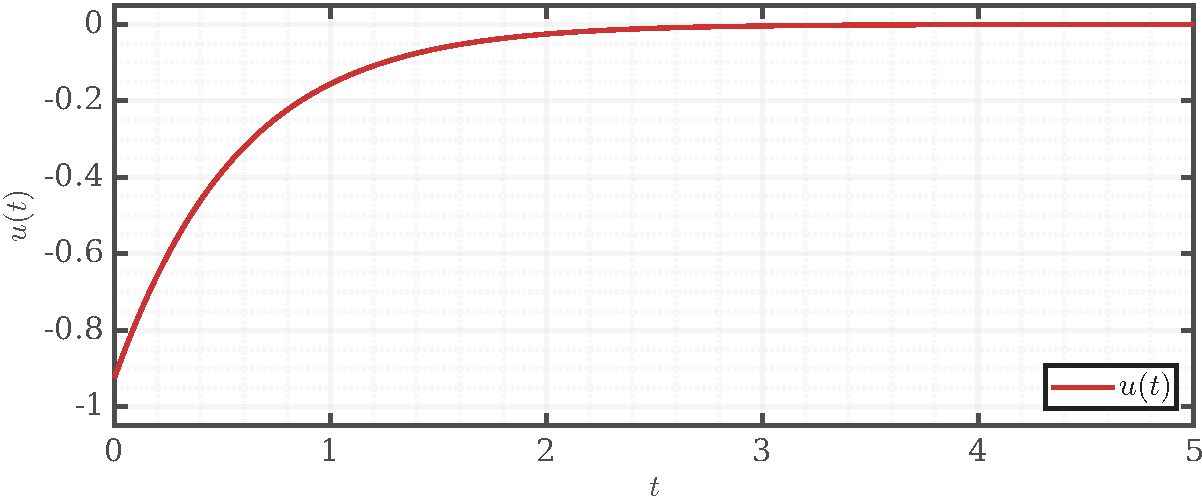
\includegraphics[width=0.65\textwidth]{../images/task4/u_2.pdf}
		\caption{Управление \(u(t)\): эксперимент 2 ($Q^*, r=10$)}
	\end{figure}
	
	\begin{figure}[H]
		\centering
		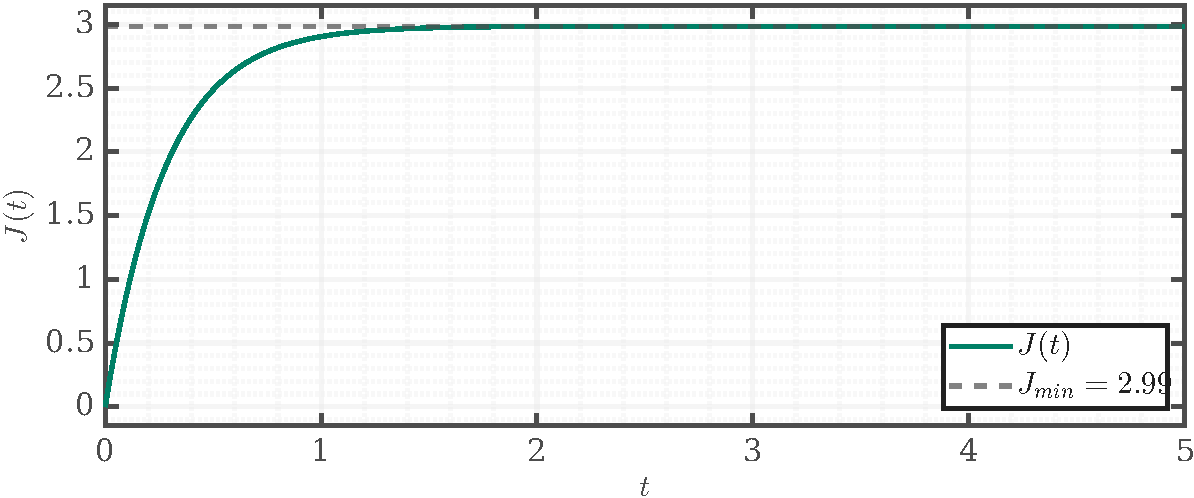
\includegraphics[width=0.65\textwidth]{../images/task4/J_2.pdf}
		\caption{Критерий качества \(J(t)\): эксперимент 2 ($Q^*, r=10$)}
	\end{figure}
	
	% --- Эксперимент 3 ---
	\begin{figure}[H]
		\centering
		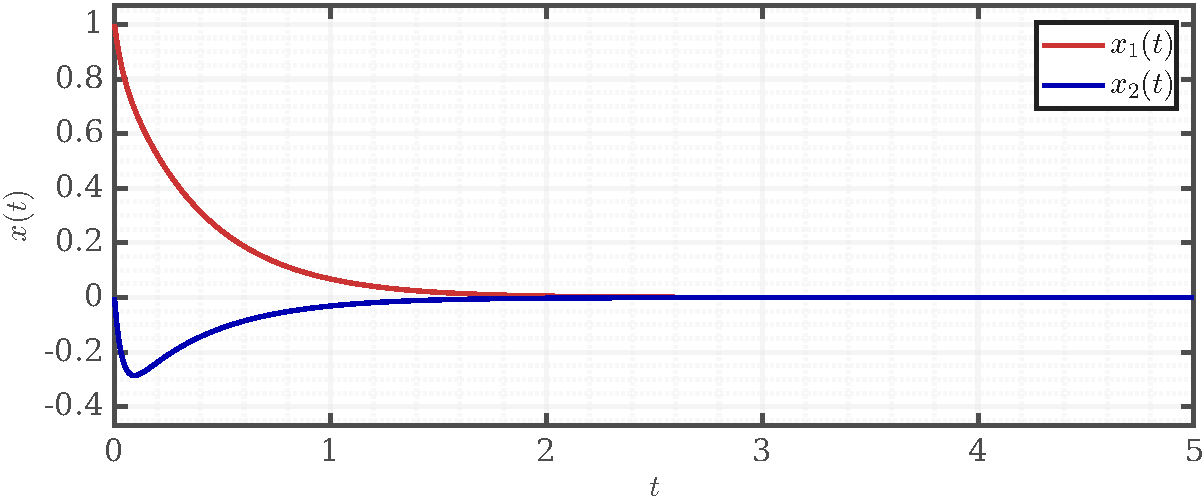
\includegraphics[width=0.65\textwidth]{../images/task4/x_3.pdf}
		\caption{Траектории состояния \(x(t)\): эксперимент 3 ($5Q^*, r=0.5$)}
	\end{figure}
	
	\begin{figure}[H]
		\centering
		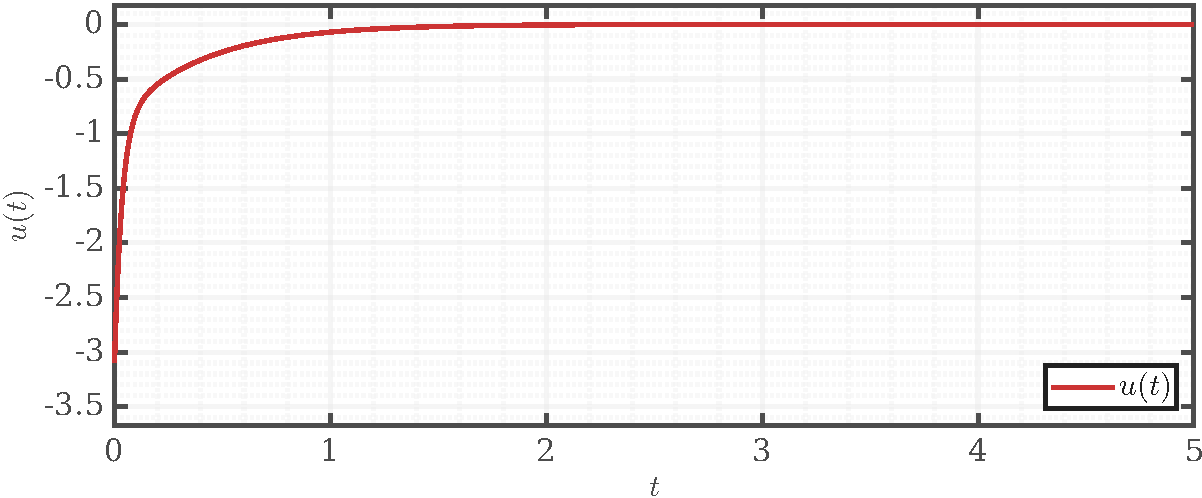
\includegraphics[width=0.65\textwidth]{../images/task4/u_3.pdf}
		\caption{Управление \(u(t)\): эксперимент 3 ($5Q^*, r=0.5$)}
	\end{figure}
	
	\begin{figure}[H]
		\centering
		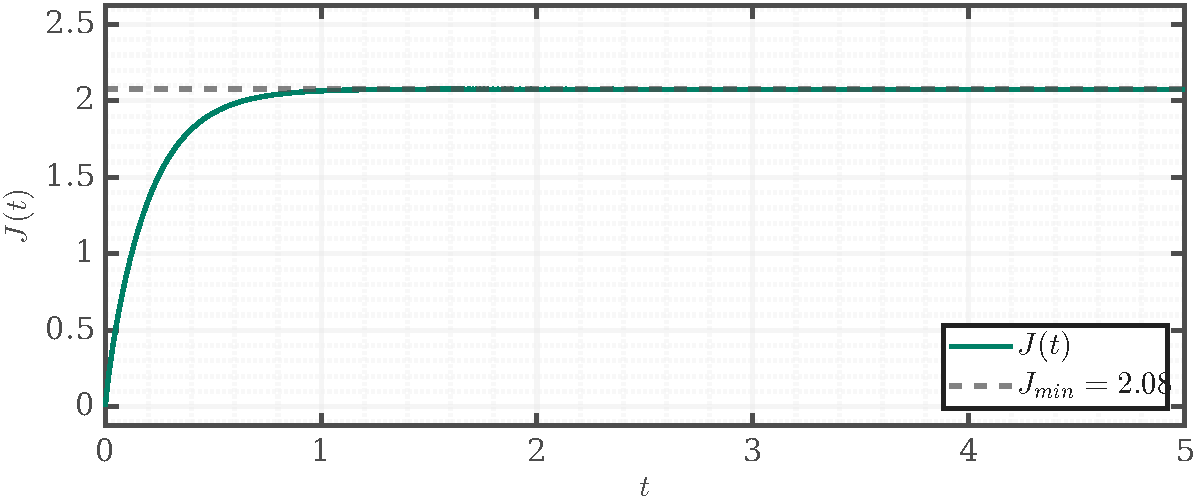
\includegraphics[width=0.65\textwidth]{../images/task4/J_3.pdf}
		\caption{Критерий качества \(J(t)\): эксперимент 3 ($5Q^*, r=0.5$)}
	\end{figure}
	
	 Анализ результатов показывает, что при пропорциональном увеличении весов ($Q \to 2Q$, $r \to 2r$) траектории $x(t)$ и управление $u(t)$ не изменяются, а значение критерия возрастает ровно в два раза. 
	 
	 Увеличение штрафа за управление ($r=10$) снижает энергозатраты ценой замедления скорости компонент. 
	 
	 Напротив, снижение $r$ до $0.5$ делает регулятор агрессивным: переходный процесс ускоряется.
	
	

	
	\newpage
	\section{Вывод}
	Синтезированный на основе уравнения Риккати LQR-регулятор обеспечивает асимптотическую устойчивость замкнутой системы и минимизацию квадратичного критерия качества при точном задании весовых параметров. Анализ робастности подтвердил, что оптимальное управление является глобальным минимумом функционала.
	

	
	
	
	
	
	
	
	
	
	
	
	
	
	\newpage
	\section{Приложение}
	
	\begin{lstlisting}[caption={Синтез матрицы регулятора}, label=lst:icare]
clc; clear;

A = [0 1; 5 -3];
b = [2; 5];
x0 = [1;0];

Q = [2 0; 0 3];
r = 2;

[P, ~, ~] = icare(A, b, Q, r);

K = r^-1 * b' * P;
eig(A - b*K);

J_min = x0' * P * x0;

\end{lstlisting}
	
\end{document}